%\documentclass[12pt]{article}

\usepackage{tikz}
\usepackage{mathtools}
\usepackage{xcolor}
\usetikzlibrary{arrows,automata,positioning}
\usetikzlibrary{arrows.meta,positioning}
\definecolor{darkgreen}{rgb}{0.0, 0.5, 0.0}
%\begin{document}

% images:
% \maxIndependentSet
% \maxFlow
% \mvcInsufficient
% \mvcSufficient
% \chromaticNumber
% \exampleLPConstraints
% \primalSimplexExample
% \milpExample


% adapted from https://tex.stackexchange.com/questions/341949/how-to-plot-a-network-flow-with-tikz
\newcommand{\maxFlow}{
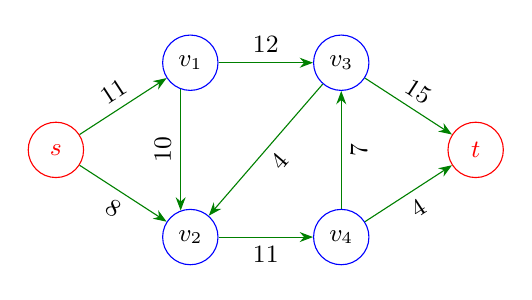
\begin{tikzpicture}[
      mycircle/.style={
         circle,
         draw=blue,
         text opacity=1,
         inner sep=0pt,
         minimum size=20pt,
         font=\small},
      myarrow/.style={-Stealth, draw=darkgreen},
      node distance=0.6cm and 1.2cm
      ]
      \node[mycircle, red] (c1) {$s$};
      \node[mycircle,below right=of c1] (c2) {$v_2$};
      \node[mycircle,right=of c2] (c3) {$v_4$};
      \node[mycircle,above right=of c1] (c4) {$v_1$};
      \node[mycircle,right=of c4] (c5) {$v_3$};
      \node[mycircle,below right=of c5, red] (c6) {$t$};

    \foreach \i/\j/\txt/\p in {% start node/end node/text/position
      c1/c2/8/below,
      c1/c4/11/above,
      c2/c3/11/below,
      c3/c6/4/below,
      c4/c5/12/above,
      c5/c6/15/above,
      c5/c2/4/below,
      c3/c5/7/below}
       \draw [myarrow] (\i) -- node[sloped,font=\small,\p] {\txt} (\j);


     % draw this outside loop to get proper orientation of 10
     \draw [myarrow] (c4.250) -- node[sloped,font=\small,above,rotate=180] {10} (c2.110);
¸\end{tikzpicture}
}

\newcommand{\mvcInsufficient}{
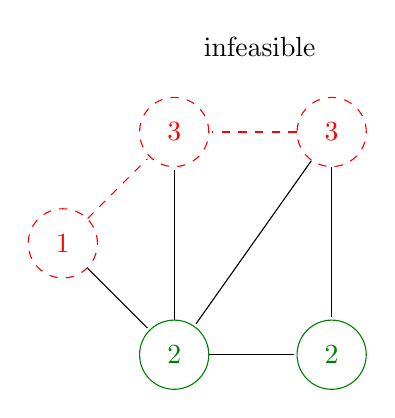
\begin{tikzpicture}[shorten >=1pt,node distance=2cm,on grid,auto]

\node[state,red, dashed] (x1)                      	 {$1$};
\node[state, darkgreen] (x2)[below right of=x1]	 {$2$};
\node[state, red, dashed] (x3)[above right of=x1]	 {$3$};
\node[state, darkgreen] (x4)[right of=x2]		 {$2$};
\node[state, red, dashed] (x5)[right of=x3]	 	 {$3$};

\path[-]
    (x1)	edge node {} (x2)
    (x2)	edge node {} (x4)
    		edge node {} (x3)
    (x5)	edge node {} (x4)
    		edge node {} (x2);

\path[-, dashed, red]
    (x1)		edge node [dashed, red] {} (x3)
    (x5)	edge node [dashed, red] {} (x3);
    
\node[] at (2.5,2.5) {infeasible};
\end{tikzpicture}
}

\newcommand{\mvcSufficient}{
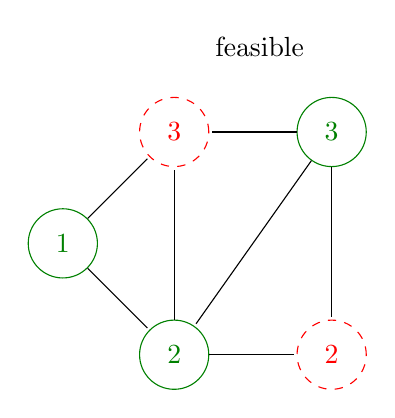
\begin{tikzpicture}[shorten >=1pt,node distance=2cm,on grid,auto]

\node[state,darkgreen]    (x1)                       {$1$};
\node[state, darkgreen]   (x2)[below right of=x1]	 {$2$};
\node[state, red, dashed] (x3)[above right of=x1]	 {$3$};
\node[state, red, dashed] (x4)[right of=x2]		     {$2$};
\node[state, darkgreen]   (x5)[right of=x3]	 	     {$3$};

\path[-]
    (x1)	edge node {} (x2)
    		edge node {} (x3)
    (x2)	edge node {} (x4)
    		edge node {} (x3)
    (x5)	edge node {} (x3)
    		edge node {} (x4)
    		edge node {} (x2);
    		
\node[] at (2.5,2.5) {feasible};
\end{tikzpicture}
}

\newcommand{\chromaticNumber}{
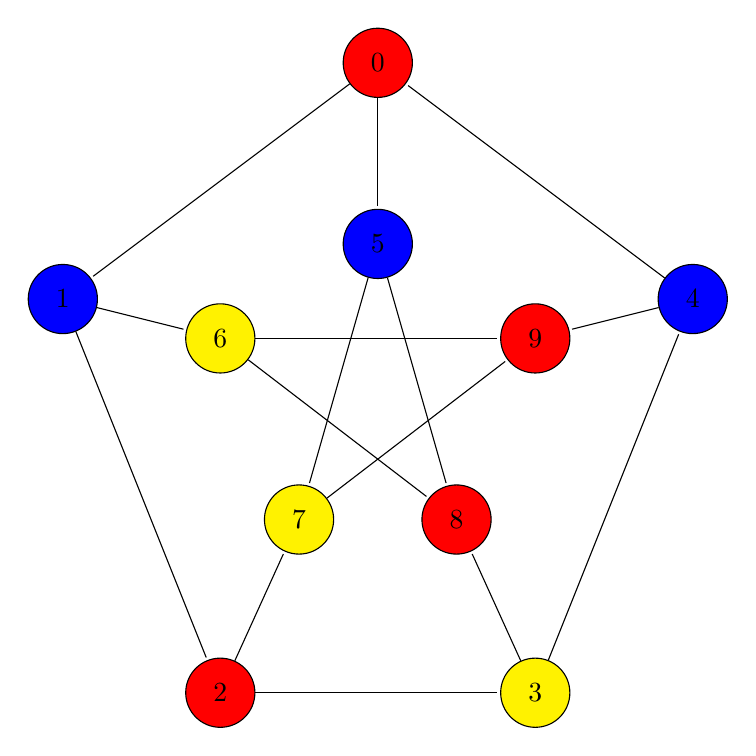
\begin{tikzpicture}[shorten >=1pt,node distance=2cm,on grid,auto, draw=black]

\node[state,fill=red]    (x0) at (5,9)                     {$0$};
\node[state,fill=blue]    (x1) at (1,6)                    {$1$};
\node[state,fill=red]    (x2) at (3,1)                     {$2$};
\node[state,fill=yellow]    (x3) at (7,1)               {$3$};
\node[state,fill=blue]    (x4) at (9,6)                    {$4$};

\node[state,fill=blue]    (x5)  at (5,6.7)                 {$5$};
\node[state,fill=yellow]    (x6)  at (3,5.5)            {$6$};
\node[state,fill=yellow]    (x7)  at (4,3.2)            {$7$};
\node[state,fill=red]    (x8)  at (6,3.2)                  {$8$};
\node[state,fill=red]    (x9) at (7,5.5)                   {$9$};

\foreach \f/\t in {% start node/end node
	 x0/x5,
	 x1/x6,
	 x2/x7,
	 x3/x8,
	 x4/x9,
	 x0/x1,
	 x1/x2,
	 x2/x3,
	 x3/x4,
	 x4/x0,
	 x5/x7,
	 x5/x8,
	 x6/x8,
	 x6/x9,
	 x7/x9}
	\path[-, draw=black]  (\f) edge node {} (\t);

\end{tikzpicture}
}

\newcommand{\maxIndependentSet}{
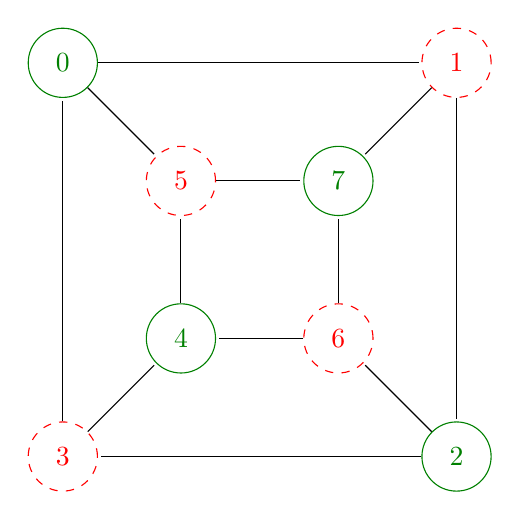
\begin{tikzpicture}[shorten >=1pt,node distance=2cm,on grid,auto, draw=black]

\node[state,darkgreen]    	(x0) at (0,5)               {$0$};
\node[state,red, dashed]    	(x1) at (5,5)               {$1$};
\node[state,darkgreen]    	(x2) at (5,0)               {$2$};
\node[state,red, dashed]  (x3) at (0,0)               {$3$};


\node[state,darkgreen]    	(x4) at (1.5,1.5)            {$4$};
\node[state,red, dashed]    	(x5) at (1.5,3.5)            {$5$};
\node[state,red, dashed]    	(x6) at (3.5,1.5)            {$6$};
\node[state,darkgreen]  (x7) at (3.5,3.5)            {$7$};



\foreach \f/\t in {% start node/end node
	 x0/x1,
	 x1/x2,
	 x2/x3,
	 x3/x0,
	 x4/x5,
	 x5/x7,
	 x6/x7,
	 x6/x4,
	 x3/x4,
	 x0/x5,
	 x1/x7,
	 x2/x6}
	\path[-]  (\f) edge node {} (\t);

\end{tikzpicture}
}


\newcommand{\drawLine}[4]{
\draw [darkgreen, line width=0.5mm] (#1,#2)--(#3,#4);
}
\newcommand{\drawDashedLine}[4]{
\draw [red, line width=0.2mm, dashed] (#1,#2)--(#3,#4);
}

% parts of a tikz picture for an example LP
\newcommand{\exampleLP}{
\draw [help lines, gray, line width=0.02mm] (0,0) grid (5,4);

% Euclidean
\draw [->](0,0)--(0,4) node[right]{$y$};
\draw [->](0,0)--(5,0) node[right]{$x$};

% draw ticks and its labels
\foreach \x/\xtext in {1/1, 2/2, 3/3, 4/4, 5/5}
{\draw (\x cm,1pt ) -- (\x cm,-1pt ) node[anchor=north] {$\xtext$};}
\foreach \y/\ytext in {1/1, 2/2, 3/3, 4/4}
{\draw (1pt,\y cm) -- (-1pt ,\y cm) node[anchor=east] {$\ytext$};}

\drawLine{2}{3}{3}{3}
\drawDashedLine{3}{3}{5}{3}
\drawDashedLine{0}{3}{2}{3}

\drawLine{0}{2}{2}{3}
\drawDashedLine{2}{3}{4}{4}

\drawLine{0}{0}{0}{2}
\drawDashedLine{0}{2}{0}{4}

\drawLine{0}{0}{5}{0}

\drawLine{5}{0}{4}{2}
\drawDashedLine{4}{2}{3}{4}

\drawLine{4}{2}{3}{3}
\drawDashedLine{4}{2}{5}{1}
\drawDashedLine{2}{4}{3}{3}

% objective function
\draw [cyan, line width=0.5mm] (1,4)--(5,2);
\coordinate[label = above right:\textcolor{cyan}{max}]() at (1.625,3.625);
\draw [dashed,->,>=stealth, line width=0.5mm, cyan] (1.375,3.5) -- (1.5,3.75);
\draw [dashed,->,>=stealth, line width=0.5mm, cyan] (4.375,2) -- (4.5,2.25);
}

% MILP example
\newcommand{\milpExample}{
\begin{tikzpicture}[scale=1]
\exampleLP

\foreach \x/\y in {0/0, 1/0, 2/0, 3/0, 4/0, 5/0, 0/1, 1/1, 2/1, 3/1, 4/1, 0/2, 1/2, 2/2, 3/2, 4/2, 2/3, 3/3}
{\node at (\x,\y) [circle,fill, blue,inner sep=1.5pt]{}; }
\end{tikzpicture}
}

\newcommand{\drawArrowLine}[4]{
\draw [blue, line width=0.5mm, -stealth] (#1,#2)--(#3,#4);
}
\newcommand{\primalSimplexExample}{
\begin{tikzpicture}[scale=1,]
\exampleLP


\foreach \i/\x/\y in {1/0/0, 2/5/0, 3/3.25/1.25, 4/2.25/2.25}
{\coordinate[label = above right:$(\i)$]() at (\x,\y);}

\foreach \i/\x/\y in {1/0/0, 2/5/0, 3/4/2, 4/3/3}
{\node at (\x,\y) [circle,fill, black,inner sep=2pt](x){};}
\drawArrowLine{0}{0}{5}{0}
\drawArrowLine{5}{0}{4}{2}
\drawArrowLine{4}{2}{3}{3}
\end{tikzpicture}
}

\newcommand{\exampleLPConstraints}{
\begin{tikzpicture}[scale=1]
\exampleLP


\foreach \i/\x/\y in {1/0/0.5, 2/2/0, 3/1/2, 4/2.1/2.3, 5/2.9/1.9, 6/3.8/0.4}
{\coordinate[label = above right:\rProp{\i}]() at (\x,\y); }

\end{tikzpicture}
}

%\end{document}